\section{QoI Model}
\label{sec:qoi_model}

Let us define the following terms:

\begin{itemize}
  \item $W$ = Channel Rate (bits/second)
  \item $T$ = Timeliness Requirement (seconds)
  \item $k_{req}$ = Number of required images
  \item $I_S$ = Size of each image (bits)
  \item $CF$ = Channel Factor
  \item $TF$ = Traffic Factor
  \item $P_S$ = Packet size
  \item $DF$ = Delay Factor
  \item $PL$ = Path Length
  \item $p_{i,j}$ = Probability of a flow from $i$ to $j$
\end{itemize}

In the conference submission we derived the following equation for scalability that uses each of these defined terms:
\begin{equation}
	W \cdot T - k_{req} \cdot I_S \cdot CF \cdot TF - P_S \cdot DF \cdot (PL-1) \geq 0	
\end{equation}

If we rearrange this equation, we can view the satisfiability of timeliness in terms of delay components:
\begin{equation}
	T \geq \frac{ k_{req} \cdot I_S \cdot CF \cdot TF}{W} + \frac{P_S \cdot DF \cdot (PL-1)}{W}
\end{equation}

In our previous analysis, we strive to determine the limits of this timeliness satisfiability by utilizing some static values and some average values where appropriate in this relation.  The resulting analysis provided approximate values for QoI satisfiability and network scalability, but what if we want to expand satisfiability to a stochastic definition?  And/or can we provide more accurate estimations by using more detailed models of the actual values of the parameters in the above list? 

To begin answering these questions, we can look at some of these parameters in more detail and use more accurate descriptions of them by classifying them as Random Variables with appropriate probability density distributions.  In this case, we start by examining a line network.  Its simple structure and routing make it a nice, simple topology to use as an exploratory model.  Here, the same traffic model as in the conference submission is also used.  In this model, each node is a source of a query that is delivered to a randomly chosen destination.  

\subsection{Traffic Factor}

Let $\rho(x)$ be the number of shortest paths of all other nodes that include node $x$ (NOTE: Is this the same as Betweeness Centrality?).  Let $F_{ij}$ be represent the existence of a flow existing from node $i$ to node $j$.  We assume that $F_{ij}$ is equal to $1$ with probability $p_f$ and $0$ otherwise.  Then, the traffic factor of a node $x$, $R_x$, is given by the sum of $F_{ij}$ for all $\rho(x)$ pairs $(i,j)$ in which $x$ is along the shortest path.  Assuming that $F_{ij}$ is i.i.d. for all pairs $(i,j)$, then $R_x$ can be approximated by a Normal RV with mean $\rho(x) p_f$ and variance $\rho(x) p_f (1-p_f)$:

\begin{equation}
	f_{R_x} = \mathcal{N}(\rho(x) p_f, \rho(x) p_f (1-p_f)) 
\end{equation}

Let's consider a flow originating at node $i$, and call the destination of the flow $j$.  When characterizing the largest contributor to delay, we need to determine the maximum expected Traffic Factor through which the flow will be forwarded.  We will use $TF_{i}$ to represent that maximum expected Traffic Factor for a flow with origin $i$.  To get a distribution for overall delay, we want to derive a distribution for this value.  We will use $P_{TF_i}$ to represent the PDF of the Traffic Factor for this flow originating at node $i$.  
We need to first find the node that has the largest expected TF between node $i$ and node $j$, so we need to find the node $x'$ that has the maximum expected TF.  Since $p_f$ is constant, the node with the maximum expected TF is:

\begin{equation}
\label{eq:max_tf_node}
	x' = \argmax_{x = [\min(i,j), \max(i,j)]} \rho(x) 
\end{equation}

Then, we can say that the distribution of the TF for this flow would be

\begin{equation}
	f_{TF_{i}}(tf) = \mathcal{N}(\rho(x') p_f, \rho(x') p_f (1-p_f))
	\label{eq:pdf_TF_1}
\end{equation}

Given a network graph, values of $\rho(x)$ and the solution of ($\ref{eq:max_tf_node}$) could be analytically determined for that specific case.  In networks with regular structure, though, we may be able to develop closed form expressions for 

\subsection{Path Length}

%\begin{figure}
%\begin{centering}
%    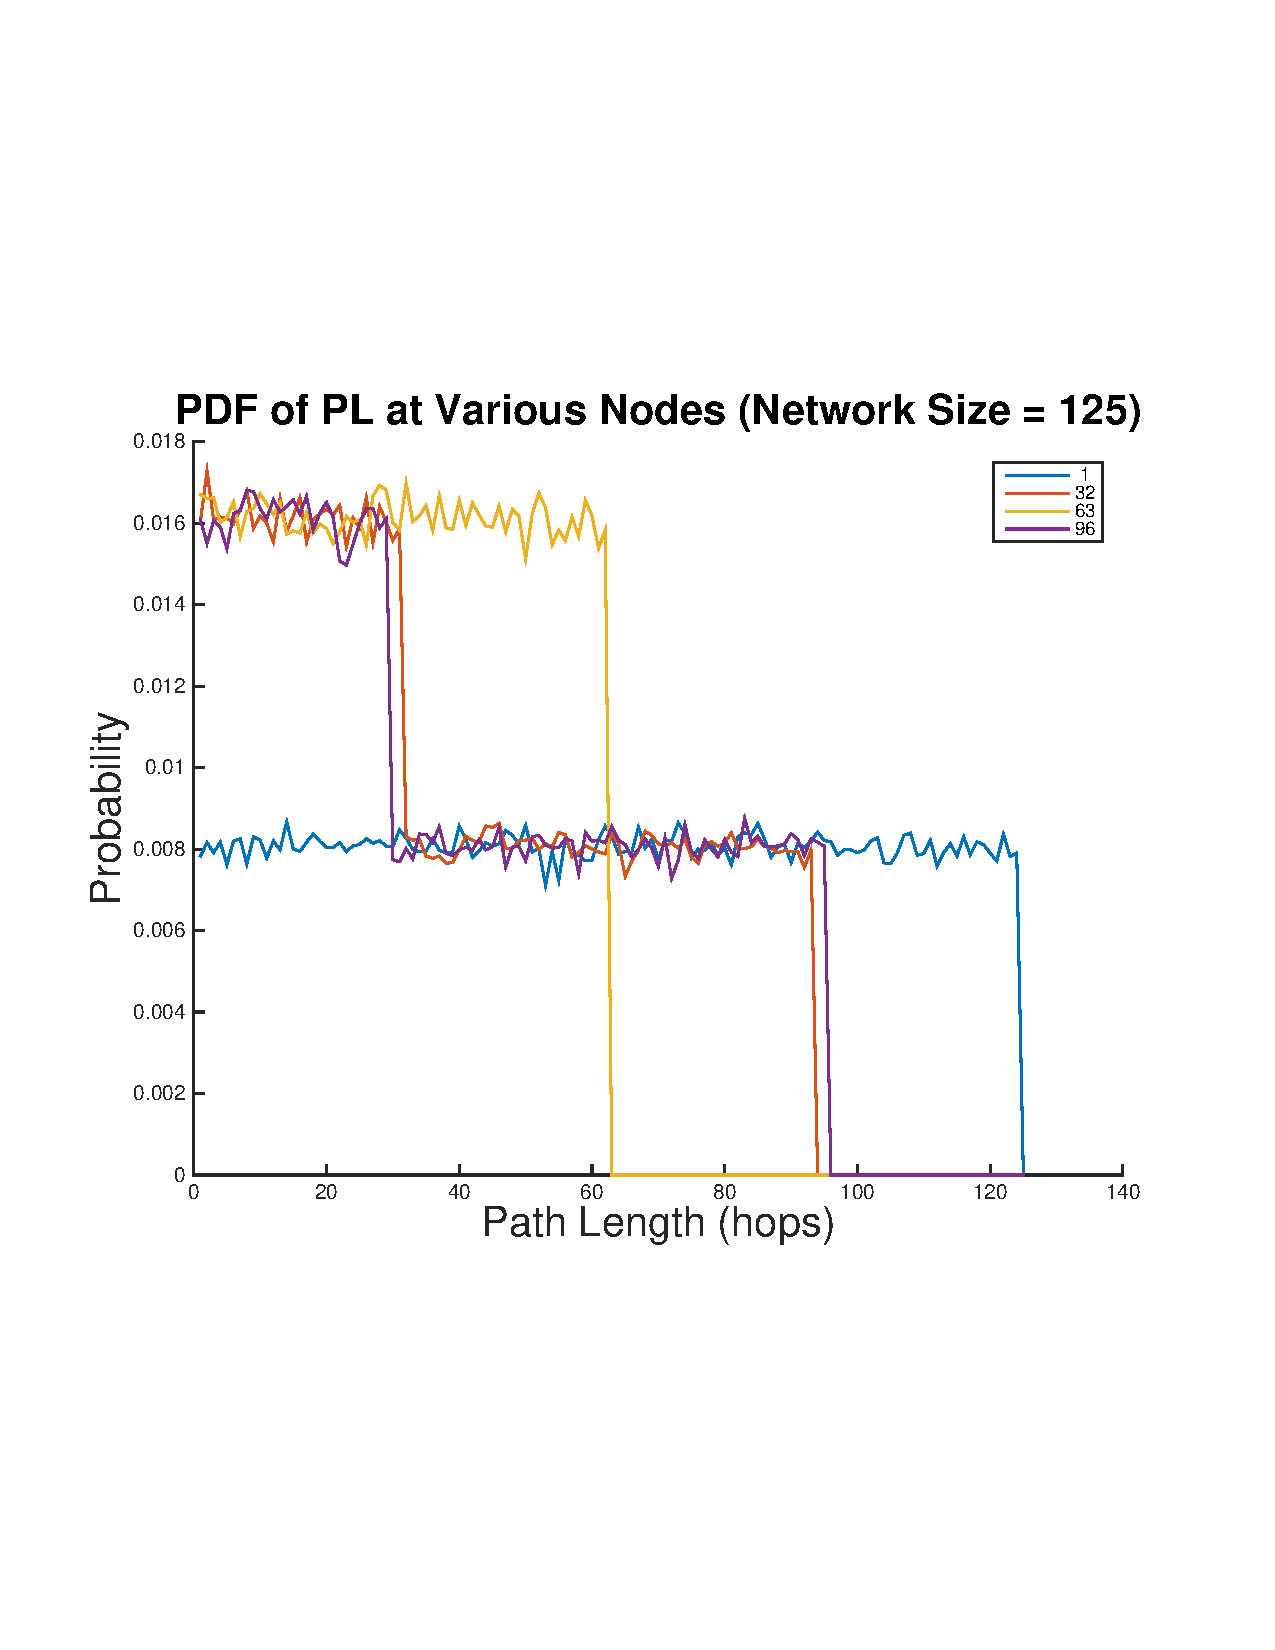
\includegraphics[scale=0.4, clip=true, trim=15mm 65mm 20mm 65mm]{figures/PL_PDFs_each_node_line_net_125.pdf}
%    \caption{Plotting the frequency of experienced Path Lengths for different node positions in a line network shows that PL can be modeled as disjoint Uniform Random Variables.}
%    \label{fig:PL_PDFs_line_net}
%\end{centering}
%\end{figure}
\begin{figure}
\begin{centering}
    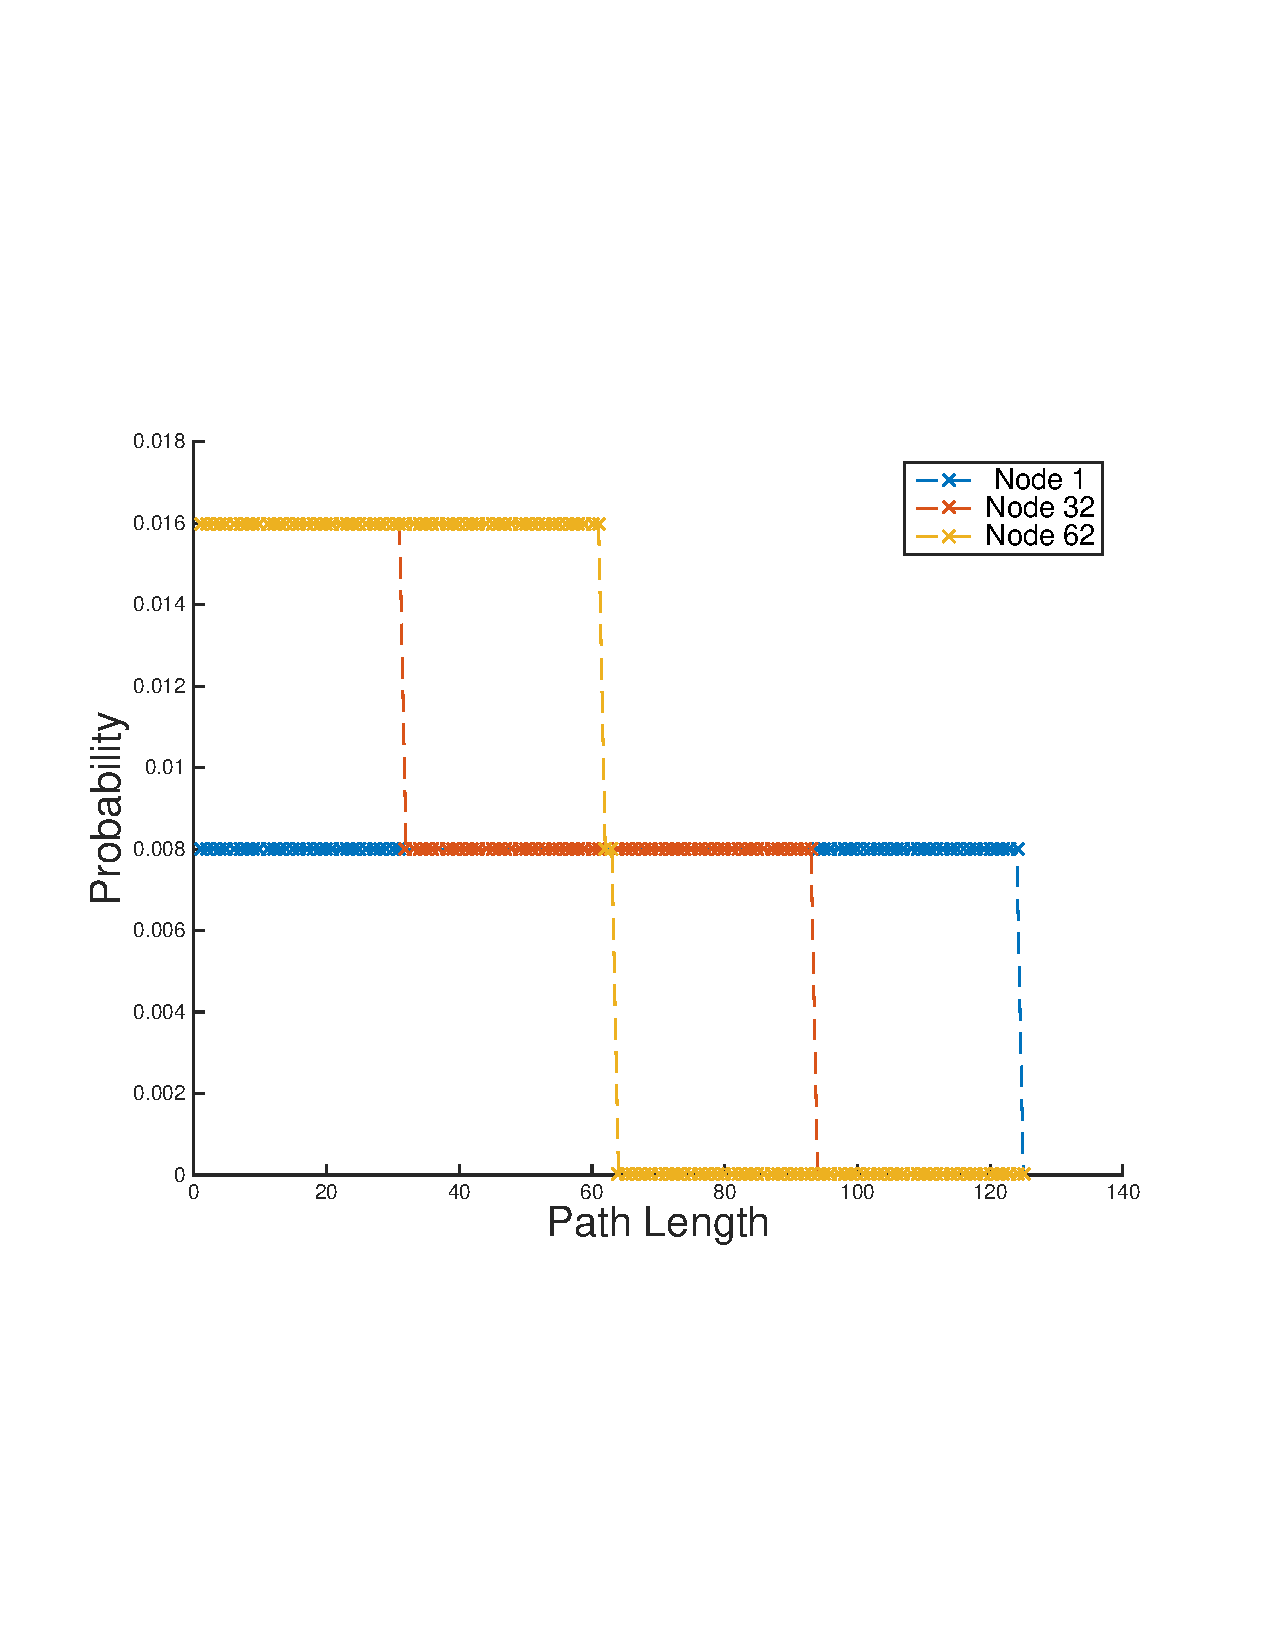
\includegraphics[scale=0.4, clip=true, trim=15mm 65mm 20mm 65mm]{figures/PDF_PL_line_net_125.pdf}
    \caption{PDF of Path Lengths for flows originating in edge cases of a line network.}
    \label{fig:PL_PDFs_line_net}
\end{centering}
\end{figure}

Next, we can capture the distribution of the path length given by flows originating in node $i$ of the network.  Once again, this distribution can be determined for any network given the topology with some simple computation, but we can provide expressions for some regular networks.


%Is the Delay Factor dependent on node position?  It must be...similar to path length, a node's position affects the probability of choosing a route with or against the flow of scheduling.  
%Finally, we can give a simple expression for the Delay Factor: 
%\begin{eqnarray*}
%	P_{DF_x}(l) &=&
%		\left\{\begin{array}{ll}
%		\frac{2}{N} & \mbox{for } 1 < l < \min(i,N-i) \\
%		\frac{1}{N} & \mbox{for } \min(i,N-i) \leq l \leq \max(i,N-i) \\
%		0 &\mbox{elsewhere}
%		\end{array}\right.
%\end{eqnarray*}


